\documentclass[a4paper, 12pt]{article}
\usepackage[portuguese]{babel}
\usepackage{chemist}
\usepackage{chemformula}
\usepackage{booktabs}
% Pacote para aceitar acentuação
\usepackage[utf8]{inputenc}
\usepackage{float}
% geometry, pacote para configurar as margens. 
% padrão ABNT => lmargin=3cm,tmargin=3cm,rmargin=2cm,bmargin=2cm
\usepackage[lmargin=3cm,tmargin=3cm,rmargin=2cm,bmargin=2cm]{geometry}

% graphicx = usar imagem (\includegraphics), comment = texto em formato de comentário, enumitem = enumeração, multirow e multicol = uso de tabelas, indentf = identar primeira linha
\usepackage{graphicx,xcolor,comment,enumitem,multirow,multicol,indentfirst}
\setlength{\parindent}{1.25cm} % não identa a primeira linha

% Pacotes para matemática
\usepackage{amsmath, amssymb, amsthm, amsfonts,  mathtools, amstext, nccmath}
\everymath{\displaystyle}

\usepackage[utf8]{inputenc}
\usepackage{hyperref}

%
% Título e autor do documento
%
\title{Química Analítica Quantitativa\\
	\large{\textbf{\\Volumetria de Neutralização \\
	Titulação de Ácidos Fracos com Base Forte (NaOH)}}
}

\author{Rogério Ribeiro Macêdo}
\date{\today}

\usepackage[font=scriptsize,labelfont=bf]{caption}
\usepackage{subcaption}
\usepackage{siunitx}

\usepackage{fancyhdr}
\fancyhf{} % limpa os cabecalhos e rodapés
\fancyhead[C]{Titulação de Ácidos Fracos com Base Forte (NaOH)} % define o cabeçalho personalizado
\renewcommand{\footrulewidth}{0.5pt}
\fancyfoot[C]{\thepage}
\pagestyle{fancy} % sem definir esse comando, o cabeçalho personalizado não é exibido
\setcounter{secnumdepth}{5}
\usepackage{titletoc}
\begin{document}

\maketitle
\tableofcontents
\newpage
\listoffigures
\newpage
\listoftables
\newpage

O presente trabalho foi realizado objetivando aplicar a sequência de cálculos necessários à titulação de ácido fraco (titulado) com uma base forte, no caso estamos usando o hidróxido de sódio (titulante) como base forte. A partir dos cálculos o resultado final é a produção da curva de titulação. Lembrando que, para tal, por se tratar de um ácido fraco faz-se necessário a utilização da constante de dissociação do ácido (Ka). \\

A curva de titulação será construída relacionando o volume adicionado de NaOH com o valor do pH resultante da titulaçao. 

Para a execução do trabalho um código escrito em Python foi utilizado na geração dos dados. O mesmo pode ser encontrado no link  \href{https://github.com/rogerioribeiromacedo/quimica/tree/main/quimica_analitica}{https://github.com/rogerioribeiromacedo}

\section{Etapas da titulação}
Antes de iniciar vale lembrar que o processo de titulação envolve basicamente 4 etapas e em cada uma delas o cálculo do pH é realizado considerando o contexto da titulação:

\begin{description}
	\item[\underline{Etapa 1}]: antes de iniciar a titulação \hfil \\ Neste ponto a solução contém apenas ácido acético. Portanto, o valor do pH é determinado pela dissociação do ácido.
	\item[\underline{Etapa 2}]: antes de atingir o ponto de equivalência \hfil \\ Ainda há ácido para reagir, assim, o pH é determinado pelo sistema tampão.
	\item[\underline{Etapa 3}]: no ponto de equivalência \hfil \\ O ponto de equivalência é o ponto onde todo o ácido reagiu com a base. O volume da base para isso é aquele que será determinado pelo volume de equivalência. O pH é determinado pela hidrólise do sal formado.
	\item[\underline{Etapa 4}]: depois do ponto de equivalência \hfil \\ Há excesso de base. O pH é determinado através desse excesso. A hidrólise do sal contribui pouco nesse ponto, pois o excesso de base reprime esta reação.
\end{description}

\section{Lista de Ácidos}

Foi realizado um levantamento de 10 ácidos (monopróticos) para que pudéssemos avaliar o comportamento da curva de titulação destes. Abaixo apresenta-se a lista destes ácidos:

\begin{table}[H]
	\begin{center}
		\caption{Lista de Ácidos Fracos}
		\label{dados_lista_acidos}
		\begin{tabular}{lp{5cm}lp{5cm}lp{5cm}lp{5cm}}\toprule
			& \textbf{Ácido} & \textbf{Fórmula} & \textbf{Ka} & \textbf{pKa} \\ \midrule
			& Ácido acético & \chemform{CH_{3}COOH} & $1,75 \times 10^{-5}$ & 4,756 \\
			& Ácido benzoico & \chemform{C_{6}H_{5}CO_{2}H} & $6,25 \times 10^{-5}$ & 4,204 \\
			& Ácido ciânico & \chemform{HCNO} & $3,50 \times 10^{-4}$ & 3,460 \\
			& Ácido fórmico & \chemform{CH_{2}O_{2}} & $1,80 \times 10^{-4}$ & 3,750 \\
			& Ácido hidrazoico & \chemform{HN_{3}}. & $2,50 \times 10^{-5}$ & 4,602 \\
			& Ácido hidrociânico & \chemform{HCN} & $6,20 \times 10^{-10}$ & 9,207 \\
			& Ácido fluorídrico & \chemform{HF} & $6,30 \times 10^{-4}$ & 3,200 \\
			& Ácido iodoacético & \chemform{CH_{2}ICO_{2}H} & $ 6,60 \times 10^{-4}$ & 3,180 \\
			& Ácido nitroso & \chemform{HNO_{2}} & $5,60 \times 10^{-4}$ & 3,252 \\
			& Ácido hipoiodoso & \chemform{HIO} & $3,20 \times 10^{-11}$ & 10,495 \\
			\bottomrule
		\end{tabular}
	\end{center}
\end{table}

\section{Dados para titulação}
Tratando-se de um experimento teórico, optou-se por considerar os dados de concentração e volume abaixo descritos. Tais valores serão utilizados para a lista de ácidos apresentada acima e também para o cálculo exemplo visto na seção  \textit{Cálculos}.

\begin{table}[H]
	\begin{center}
		\caption{Dados para titulação}
		\label{tabela_dados_titulacao}
		\begin{tabular}{lp{5cm}lp{10cm}}\toprule
			& \textbf{Ácido} & \textbf{Hidróxido de sódio} \\ \midrule			
			Volume & 50,00 mL & - \\ 
			Concentração & $0,100 \: mol \cdot L^{-1}$ & $0,100 \: mol \cdot L^{-1}$ \\ 
			\bottomrule
		\end{tabular}
	\end{center}
\end{table}

\section{Volume de equivalência}
O volume de equivalência é o volume necessário de titulante que irá reagir completamente com o titulado. No caso, o volume de NaOH necessário para reagir completamente com o ácido. O cálculo é realizado usando a expressão abaixo: 

\begin{equation*}
	V_{titulante} \times C_{titulante} = V_{titulado} \times C_{titulado}\footnote{C: concentração; V: volume}
\end{equation*}

Portanto, o volume necessário de NaOH que será necessário para neutralizar todo o ácido será de:
%\begin{fleqn}
\begin{align*}
	& V_{titulante} \times C_{titulante} = V_{titulado} \times C_{titulado} \\
	& V_{titulante} \times 0,100 = 50,00 \times 0,100 \\
	& V_{titulante} = 50,00 \text{ mL}
\end{align*}
%\end{fleqn}

No caso deste trabalho e como informado acima, a concentração do ácido e da base são as mesmas, portanto, mesmo sem realizar o cálculo já poderíamos prever que o volume necessário de base para neutralizar completamente o ácido seria de 50,00 mL.

\section{Cálculos}
A partir deste ponto realizaremos os cálculos da titulação. Como o objetivo é construir a curva de titulação, os volumes que usaremos de NaOH serão pontuais. Para a sequência de cálculos utilizaremos o \textbf{Ácido benzoico} com referência, especificamente, o seu valor de Ka que é igual a $6,25 \times 10^{-5}$.

\subsection{No ponto inicial (sem adição de NaOH)}
O valor do Ka é considerado para a realização do cálculo e este é feito usando a expressão abaixo:
%\begin{fleqn}
\begin{align*}
	Ka = \frac{[H_{3}O^{+}] \times [A^{-}]}{[HA]}
\end{align*}
%\end{fleqn}
Assim:
%\begin{fleqn}
\begin{align*}
	& Ka = \frac{x \times x}{[HA]} \longrightarrow	Ka = \frac{x^{2}}{[HA]} \rightarrow x^{2} = Ka \times [HA] \longrightarrow	x = \sqrt{Ka \times [HA]} \\ \\
	& x = [H_{3}O^{+}] = \sqrt{(6,25 \times 10^{-5}) \times 0,100} \longrightarrow	\mathbf{x = [H_{3}O^{+}] = 2,50 \times 10^{-3}}
\end{align*}
%\end{fleqn}
O valor do pH:
%\begin{fleqn}
\begin{align*}
	& pH = - \log [H_{3}O^{+}] \\
	& pH = - \log {2,50 \times 10^{-3}} \\
	& \textbf{\textcolor{red}{pH = 2,602}}
\end{align*}
%\end{fleqn}

\subsection{Antes do ponto de equivalência}
O cálculo do pH antes do ponto de equivalência faz uso da \textbf{Equação de Henderson-Hasselbalch}. Esta equação faz o relacionamento do pH de uma solução tampão, com o pKa, as concentrações da forma ácida (HA) e da base conjugada ($A^{-}$). Abaixo a equação:
%\begin{fleqn}
\begin{align*}
	pH = pKa + \frac{[A^{-}]}{[HA]}
\end{align*}
%\end{fleqn}
Portanto, precisamos do pKa do ácido benzoico:
%\begin{fleqn}
\begin{align*}
	& pKa = -log [Ka] \\
	& pKa = -log (6,25 \times 10^{-5}) \\
	& \textbf{\textcolor{red}{pka = 4,204}}
\end{align*}
%\end{fleqn}

\subsubsection{Após adição de 0,05 mL (0,00005 L) de NaOH}
Esse volume representa o volume de uma única gota de NaOH adicionada na solução do titulante. 

%\begin{fleqn}
\begin{align*}
	& [A^{-}] = \frac{ V_{NaOH} \times C_{NaOH} }{ V_{HAc} + V_{NaOH} } = \frac{0,00005 \times 0,1}{0,05 + 0,00005} \\ \\
	& \mathbf{[A^{-}] = 9,99 \times 10^{-5} \text{ \textbf{mol}} \times L^{-1}}
\end{align*}
%\end{fleqn}

%\begin{fleqn}
\begin{align*}
	& [HA] = \frac{ (C_{HA} \times V_{HA}) - (C_{NaOH} \times V_{NaOH}) }{ (V_{HA} + V_{NaOH}) } = \frac{ (0,1 \times 0,05) - (0,1 \times 0,00005) }{ (0,05 + 0,00005) }\\ \\
	& \mathbf{[HA] = 9,98 \times 10^{-2} \text{ \textbf{mol}} \times L^{-1}}
\end{align*}
%\end{fleqn}
A valor do pH:
%\begin{fleqn}
\begin{align*}
 	& pH = pKa + \log \frac{[A^{-}]}{[HA]} = 4,204 + \log \frac{(9,99 \times 10^{-5})}{(9,98 \times 10^{-2})} \\
 	& pH = 4,204 + \log (1,00 \times 10^{-3}) \\
	& pH = 4,204 + (-2,9996) \\
	& \textbf{\textcolor{red}{pH = 1,204}}
\end{align*}
%\end{fleqn}

\subsubsection{Após adição de 0,1 mL (0,0001 L) de NaOH}
%\begin{fleqn}
	\begin{align*}
		& [A^{-}] = \frac{ V_{NaOH} \times C_{NaOH} }{ V_{HA} + V_{NaOH} } = \frac{0,0001 \times 0,1}{0,05 + 0,0001} \\ \\
		& \mathbf{[A^{-}] = 1,996 \times 10^{-4} \text{ \textbf{mol}} \times L^{-1}}
	\end{align*}
%\end{fleqn}

%\begin{fleqn}
	\begin{align*}
		& [HAc] = \frac{ (C_{HA} \times V_{HA}) - (C_{NaOH} \times V_{NaOH}) }{ (V_{HA} + V_{NaOH}) } = \frac{ (0,1 \times 0,05) - (0,1 \times 0,0001) }{ (0,05 + 0,0001) }\\ \\
		& \mathbf{[HAc] = 9,96 \times 10^{-2} \text{ \textbf{mol}} \times L^{-1}}
	\end{align*}
%\end{fleqn}
O valor do pH:
%\begin{fleqn}
	\begin{align*}
		& pH = pKa + \log \frac{[A^{-}]}{[HA]} = 4,204 + \log \frac{(1,996 \times 10^{-4})}{(9,96 \times 10^{-2})} \\
		& pH = 4,204 + (-2,6981) \\
		& \textbf{\textcolor{red}{pH = 1,5059}}
	\end{align*}
%\end{fleqn}

\subsubsection{Após adição de 10,00 mL (0,01 L) de NaOH}
%\begin{fleqn}
	\begin{align*}
		& [A^{-}] = \frac{ V_{NaOH} \times C_{NaOH} }{ V_{HA} + V_{NaOH} } = \frac{0,1 \times 0,01}{0,05 + 0,01} \\ \\
		& \mathbf{[A^{-}] = 1,667 \times 10^{-2} \text{ \textbf{mol}} \times L^{-1}}
	\end{align*}
%\end{fleqn}

%\begin{fleqn}
	\begin{align*}
		& [HA] = \frac{ (C_{HA} \times V_{HA}) - (C_{NaOH} \times V_{NaOH}) }{ (V_{HA} + V_{NaOH}) } \\ \\
		& [HA] = \frac{ (0,1 \times 0,05) - (0,1 \times 0,01) }{ (0,05 + 0,01) }\\ \\
		& \mathbf{[HAc] = 6,667 \times 10^{-2} \text{ \textbf{mol}} \times L^{-1}}
	\end{align*}
%\end{fleqn}

%\begin{fleqn}
	\begin{align*}
		& pH = pKa + \log \frac{[A^{-}]}{[HA]} \\ \\
		& pH = 4,204 + \log \frac{1,667 \times 10^{-2}}{6,667 \times 10^{-2}} \\ \\
		& \textbf{\textcolor{red}{pH = 3,602}}
	\end{align*}
%\end{fleqn}

\subsubsection{Após adição de 25,00 mL (0,025 L) de NaOH}
Esse volume corresponde à metade do volume de equivalência, portanto, nesse ponto, o valor do pH corresponde ao valor do pKa. Assim:

\begin{fleqn}
	\begin{align*}
		 \textbf{\textcolor{red}{pH = pKa = 4,204}}
	\end{align*}
\end{fleqn}

\subsection{Adição de 50,00 mL (0,05 L) de NaOH - no ponto de equivalência}
A adição de 50,00 mL de base quer dizer que estamos no ponto de equivalência, onde todo o ácido é neutralizado pela base. Neste ponto, o cálculo do pH é realizado pensando-se na hidrólise do sal (NaA), cuja equação pode ser vista abaixo:

\begin{chemeqn}
	A^{-}_{(aq)} + H_{2}O_{(l)} \equilibarrow HA_{(aq)} + OH^-{} 
\end{chemeqn}

Nesse sentido, a maneira de realizar o cálculo envolverá a concentração de $OH^{-}$ presente no sistema. E outra variável que também precisaremos é o valor de Kb. Assim:

\begin{fleqn}
	\begin{align*}
		[OH^{-}] = \sqrt{Kb \times C_{NaA}}
	\end{align*}
\end{fleqn}

Para calcular a concentração do sal é preciso pensar que este tem uma relação estequiométrica de 1:1 com a base, portanto, para saber a $[A^{-}]$ usaremos os dados de NaOH, dessa forma:

%\begin{fleqn}
	\begin{align*}
		&[NaAc] = \frac{ (C_{NaOH} \times V_{NaOH}) }{ (V_{HA} + V_{NaOH}) } = \frac{ (0,1 \times 0,05) }{ (0,05 + 0,05) } \longrightarrow	 \mathbf{[NaA] = 5,0 \times 10^-2 \text{ \textbf{mol}} \times L^{-1}}
	\end{align*}
%\end{fleqn}

O próximo passo é calcular o valor do Kb: 

%\begin{fleqn}
	\begin{align*}
		&Kw = Ka \times Kb \longrightarrow	 (1,0 \times 10^{-14}) = (6,25 \times 10^{-5}) \times Kb \\ \\
		&Kb = \frac{1,0 \times 10^{-14}}{6,25 \times 10^{-5}} \longrightarrow \mathbf{Kb = 1,6 \times 10^{-10}}
	\end{align*}
%\end{fleqn}

Finalizado com o cálculo da $[OH^{-}]$ e consequentemente o valor do pH no ponto de equivalência:

%\begin{fleqn}
	\begin{align*}
		&[OH^{-}] = \sqrt{Kb \times C_{NaA}} \\
		&[OH^{-}] = \sqrt{(1,6 \times 10^{-10}) \times (5,0 \times 10^{-2})} \\
		&[OH^{-}] = 2,8286 \times 10^{-6} \longrightarrow	 pOH = 5,54 \\
		& \textbf{\textcolor{red}{pH = 8,45}}
	\end{align*}
%\end{fleqn}

\subsection{Após a adição de 50,10 mL (0,05010 L) de NaOH}
Neste ponto todo o ácido foi neutralizado, portanto, passamos a ter um excesso de base.

%\begin{fleqn}
	\begin{align*}
		&[OH^{-}] = \frac{ (C_{NaOH} \times V_{NaOH}) - (C_{HAc} \times V_{HA}) }{ (V_{NaOH} \times V_{HA}) } \\
		&[OH^{-}] = \frac{ (0,1 \times 0,05010) - (0,1 \times 0,05) }{ (0,05010 + 0,05) } \\ \\	
		&[OH^{-}] = 9,999 \times 10^{-5} \longrightarrow	pOH = 4,00004 \\
		& \textbf{\textcolor{red}{pH = 9,99996}}
	\end{align*}
%\end{fleqn}

\subsection{Resultados}
Abaixo listamos os valores iniciais e finais para o cálculo da titulação do ácido benzoico:

\begin{table}[H]
	\begin{center}
		\caption{Valores de pH nos respectivos volumes de NaOH}
		\label{dados_ac_benzoico}
		\begin{tabular}{lp{5cm}|rrp{5cm}}\toprule
			\textbf{pH} & \textbf{Volume (L)} & \textbf{pH} & \textbf{Volume (L)} \\ \midrule
			2,6020600 & 0,000000 & 2,4671600 & 0,000900 \\
			1,2044300 & 0,000050 & 2,4910800 & 0,000950 \\
			1,5059000 & 0,000100 & 2,5138000 & 0,001000 \\
			1,6824300 & 0,000150 & 2,5354400 & 0,001050 \\
			1,8078000 & 0,000200 & 2,5560800 & 0,001100 \\
			1,9051500 & 0,000250 & 2,5758300 & 0,001150 \\
			1,9847600 & 0,000300 & 2,5947600 & 0,001200 \\
			2,0521500 & 0,000350 & 2,6129400 & 0,001250 \\
			2,1105800 & 0,000400 & 2,6304100 & 0,001300 \\
			2,1621700 & 0,000450 & 2,6472500 & 0,001350 \\
			2,2083600 & 0,000500 & 2,6634900 & 0,001400 \\
			2,2502000 & 0,000550 & 2,6791800 & 0,001450 \\
			2,2884200 & 0,000600 & 12,615560 & 0,120250 \\
			2,3236300 & 0,000650 & 12,615740 & 0,120300 \\
			2,3562500 & 0,000700 & 12,615919 & 0,120350 \\
			2,3866600 & 0,000750 & 12,616099 & 0,120400 \\
			2,4151200 & 0,000800 & 12,616280 & 0,120450 \\
			2,4419000 & 0,000850 \\			
			\bottomrule
		\end{tabular}
	\end{center}
\end{table}

\subsection{Curva de Titulação}
Abaixo (Figura \ref{fig:curva_de_titulacao_ácido_benzoico}) pode-se verificar a curva de titulação do ácido benzoico.

\begin{figure}[H]
	\centering
	\includegraphics[width=0.99\linewidth]{curva/curva_de_titulacao_ácido_benzoico}
	\caption[Curva de Titulação Ácido Benzoico]{}
	\label{fig:curva_de_titulacao_ácido_benzoico}
\end{figure}


\section{Dados para as curvas titulação dos Ácidos}
Como dito no início deste documento os dados usados para a construção do gráfico foram obtidos via programa em Python. 

O programa toma como referência os dados para titulação da seção 3 e calcula o pH considerando a variação de volume do NaOH de 0,00 mL até 120 mL. A tabela abaixo apresenta a lista de ácidos com os respectivos valores de pH mínimo e máximo.

\begin{table}[H]
	\begin{center}
		\caption{Valores mínimo e máximo de pH}
		\label{tbl_vlr_minimo_maximo_pH}
		\begin{tabular}{l|rr} \toprule
			Ácido & Máximo & Mínimo \\ \midrule
			Ácido acético & 12,616280 & 1,756430 \\
			Ácido benzoico & 12,616280 & 1,204430 \\
			Ácido ciânico & 12,616280 & 0,460430 \\
			Ácido fluorídrico & 12,616280 & 0,200430 \\
			Ácido fórmico & 12,616280 & 0,750430 \\
			Ácido hidrazoico & 12,616280 & 1,602430 \\
			Ácido hidrociâncio & 12,616280 & 5,103800 \\
			Ácido hipoiodoso & 13,494570 & 5,747430 \\
			Ácido iodoacético & 12,616280 & 0,180430 \\
			Ácido nitroso & 12,616280 & 0,252430 \\
			\bottomrule
		\end{tabular}
	\end{center}
\end{table}

\section{Gráficos de Titulação}
Abaixo pode-se visualizar os gráficos resultantes dos cálculos. Nele, marcado com linha pontinhada, temos os valores do volume de equivalência e o respectivo pH para cada ácido.

\begin{figure}[H]
	\begin{subfigure}{0.5\textwidth}
		\centering
		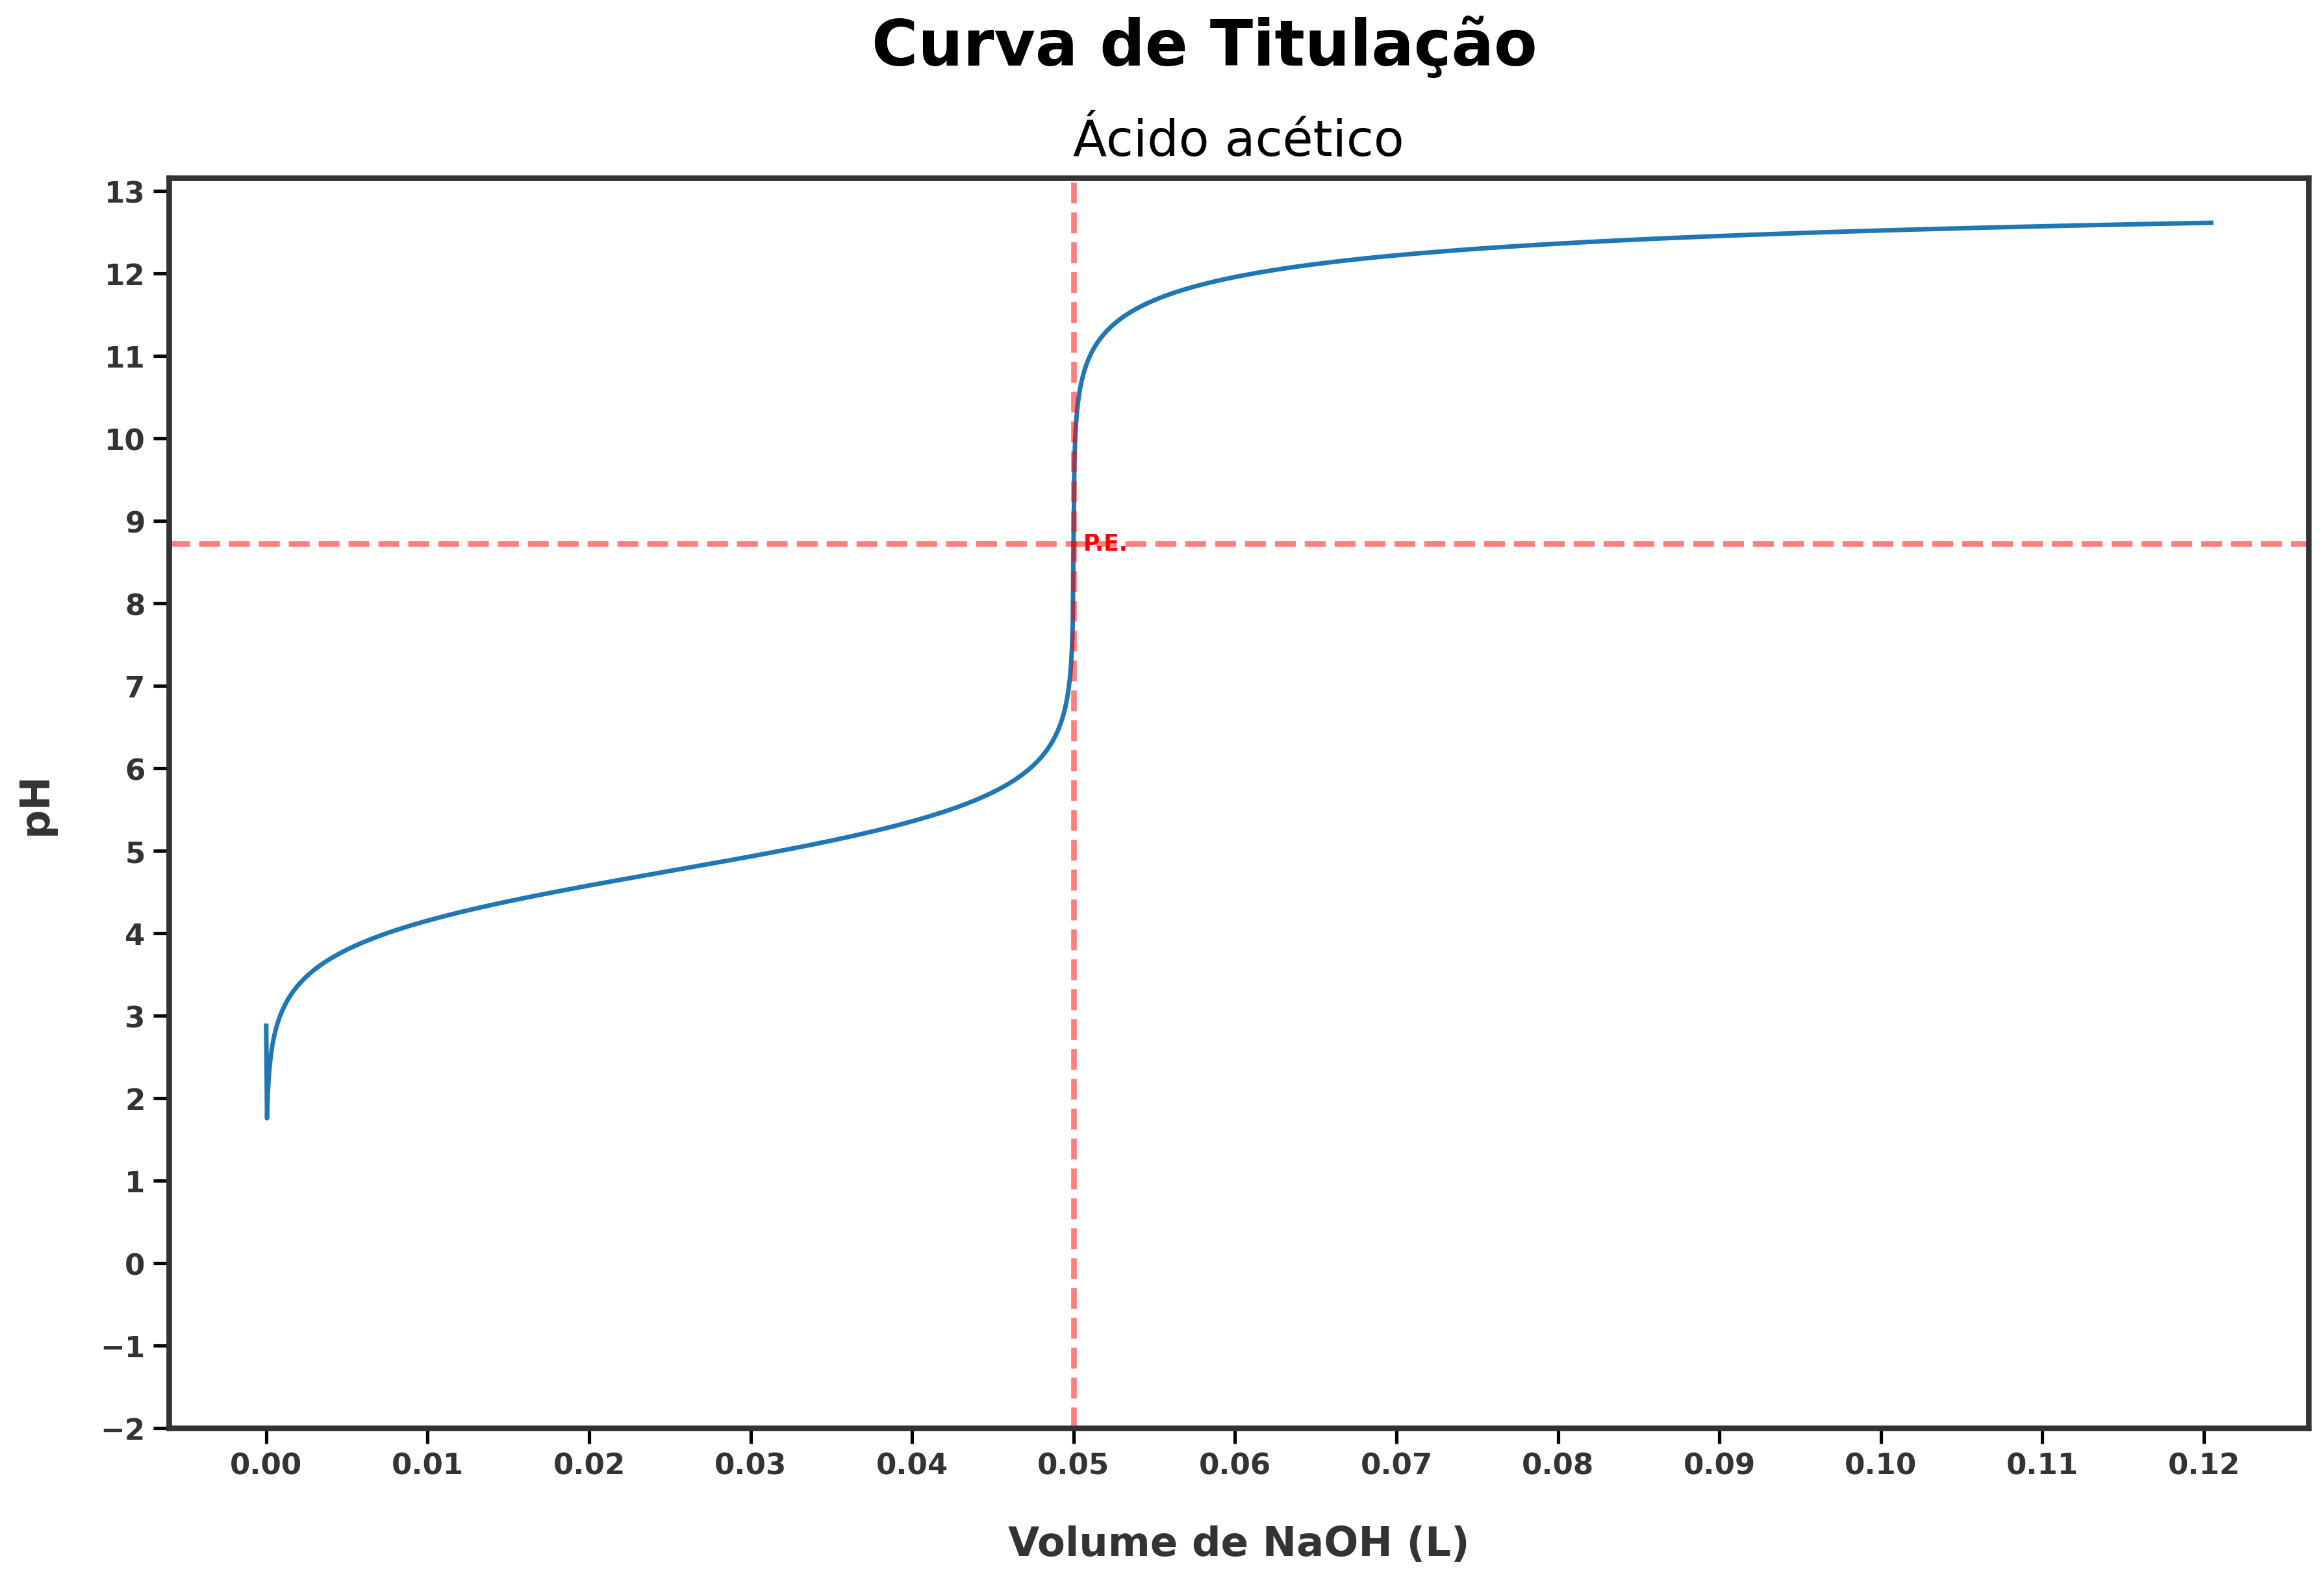
\includegraphics[width=0.9\linewidth]{curva/curva_de_titulacao_ácido_acético}
		\caption{}
		\label{fig:curvadetitulacaoacidoacetico}
	\end{subfigure}
	\begin{subfigure}{0.5\textwidth}
		\centering
		\includegraphics[width=0.9\linewidth]{curva/curva_de_titulacao_ácido_benzoico}
		\caption{}
		\label{fig:curvadetitulacaoácidobenzoico}
	\end{subfigure}
	\begin{subfigure}{0.5\textwidth}
		\centering
		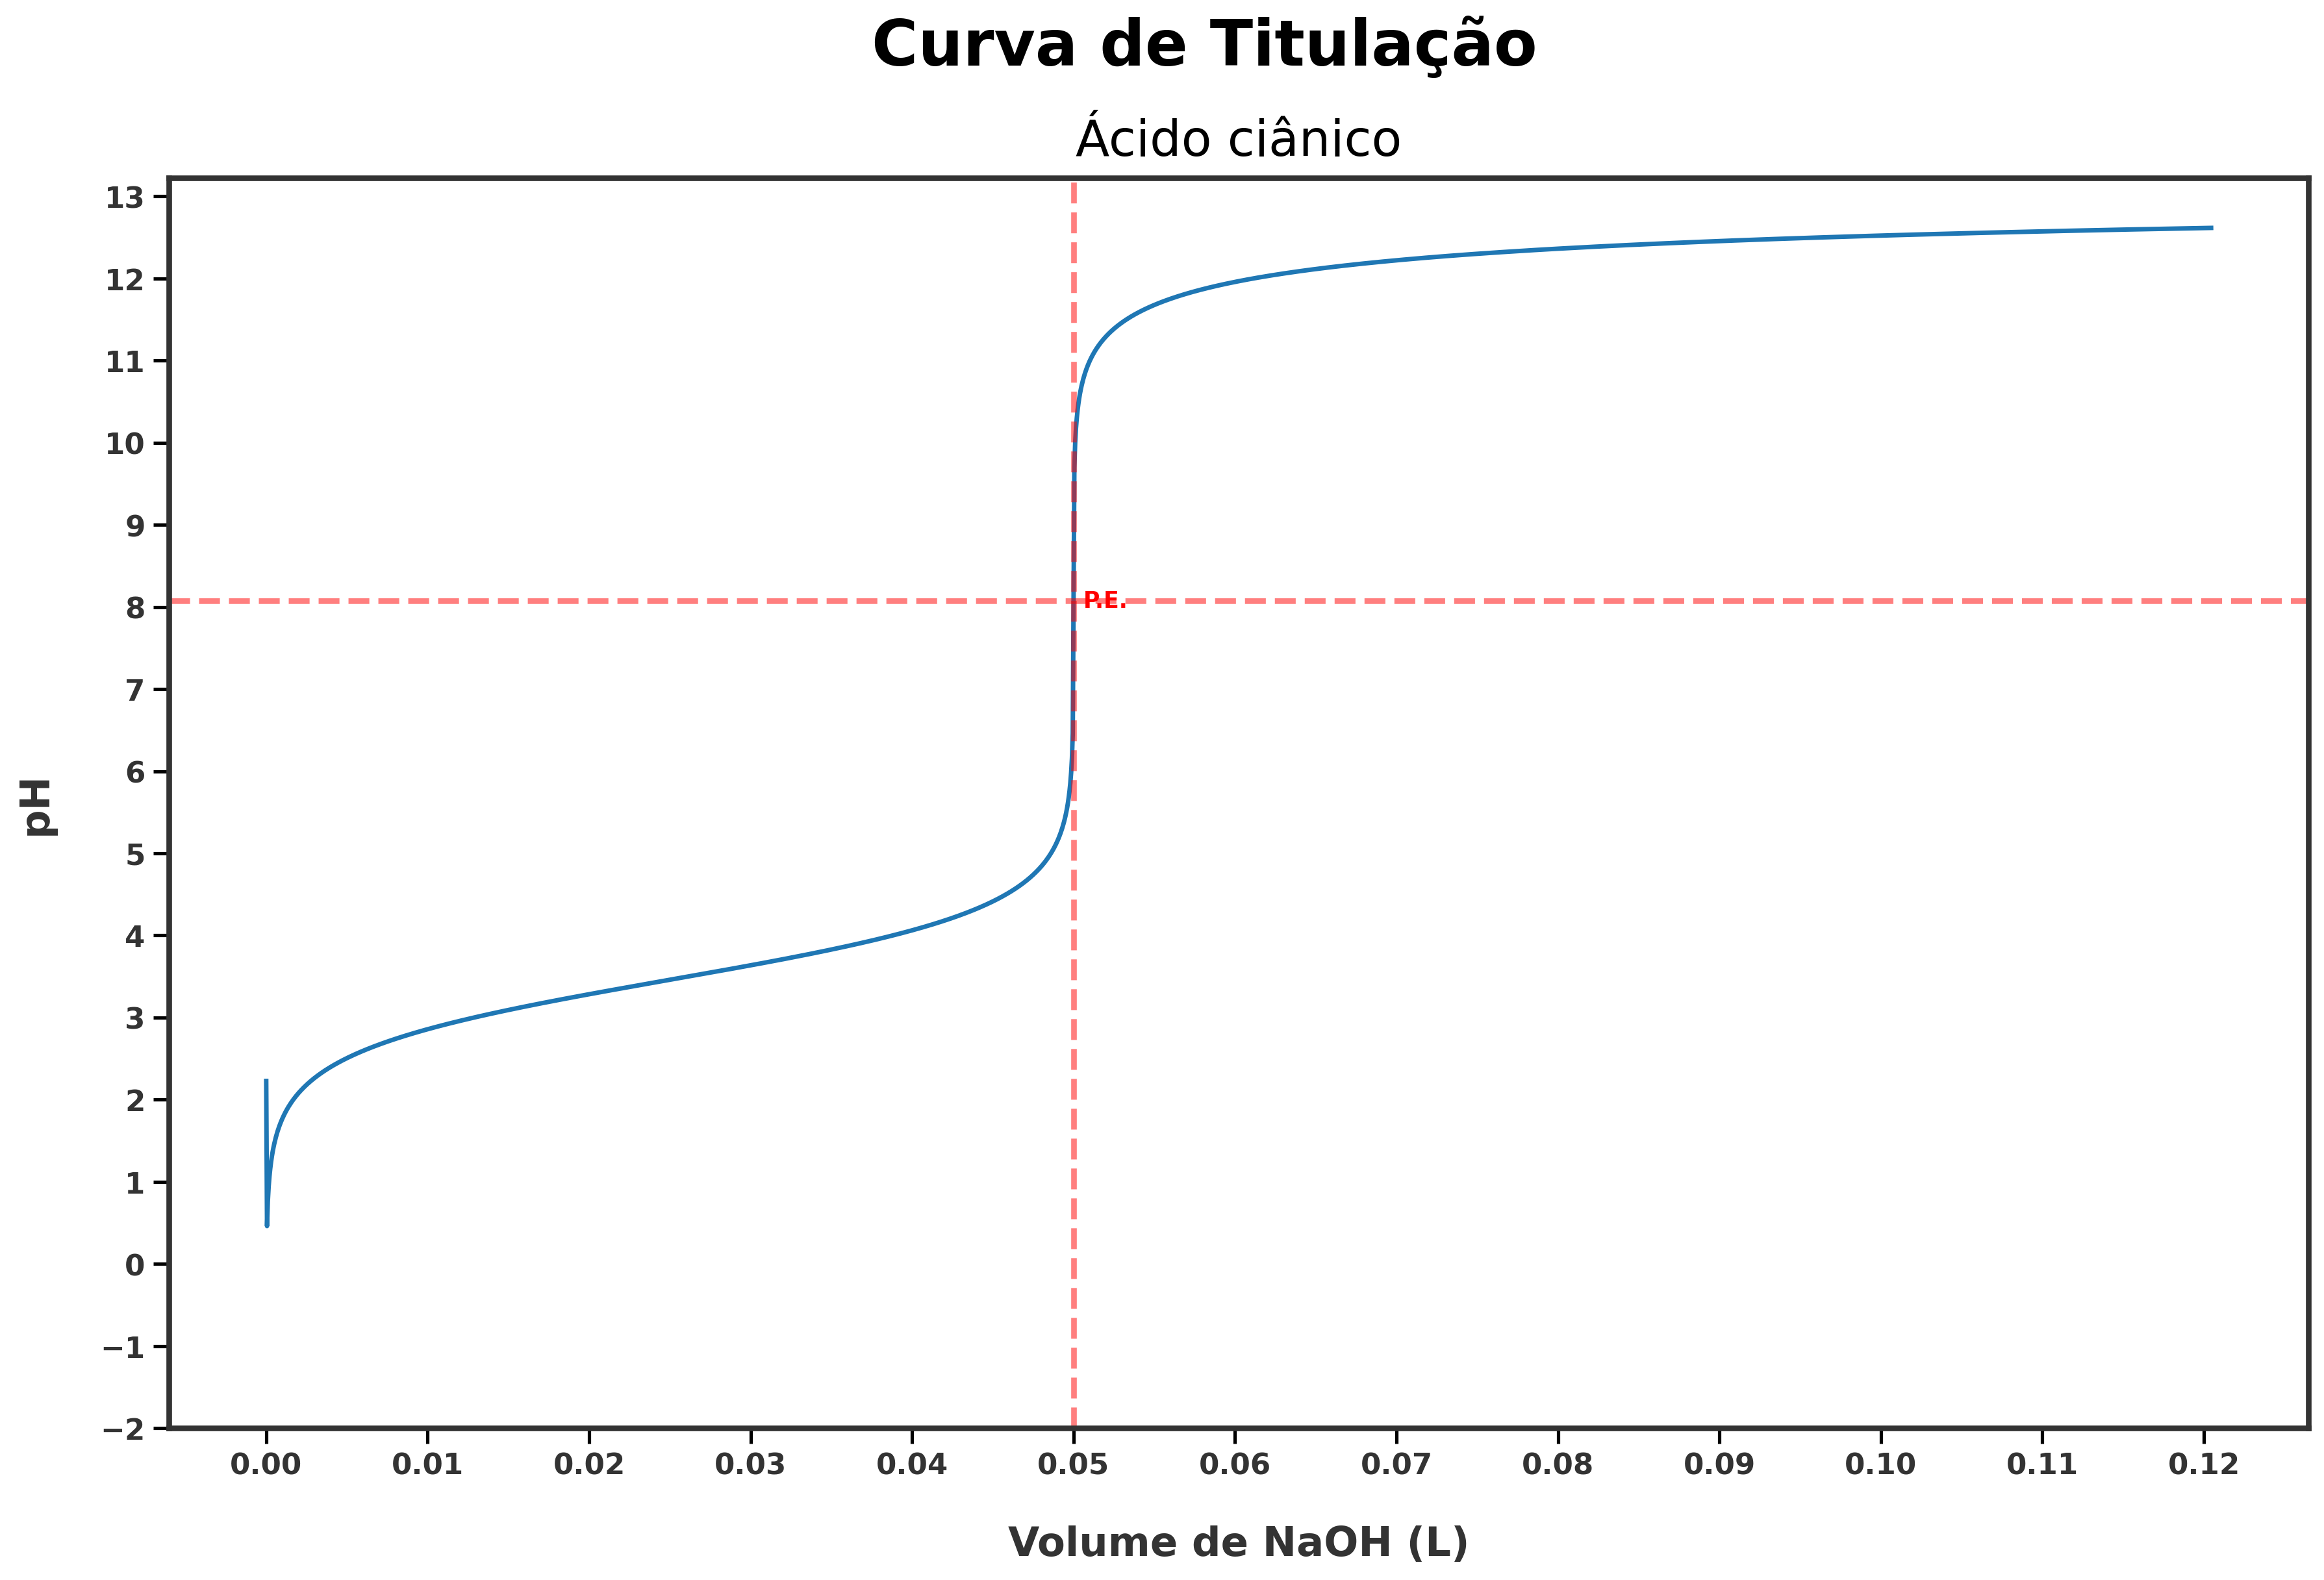
\includegraphics[width=0.9\linewidth]{curva/curva_de_titulacao_ácido_ciânico}
		\caption{}
		\label{fig:curvadetitulacaoácidociânico}
	\end{subfigure}
	\begin{subfigure}{0.5\textwidth}
		\centering
		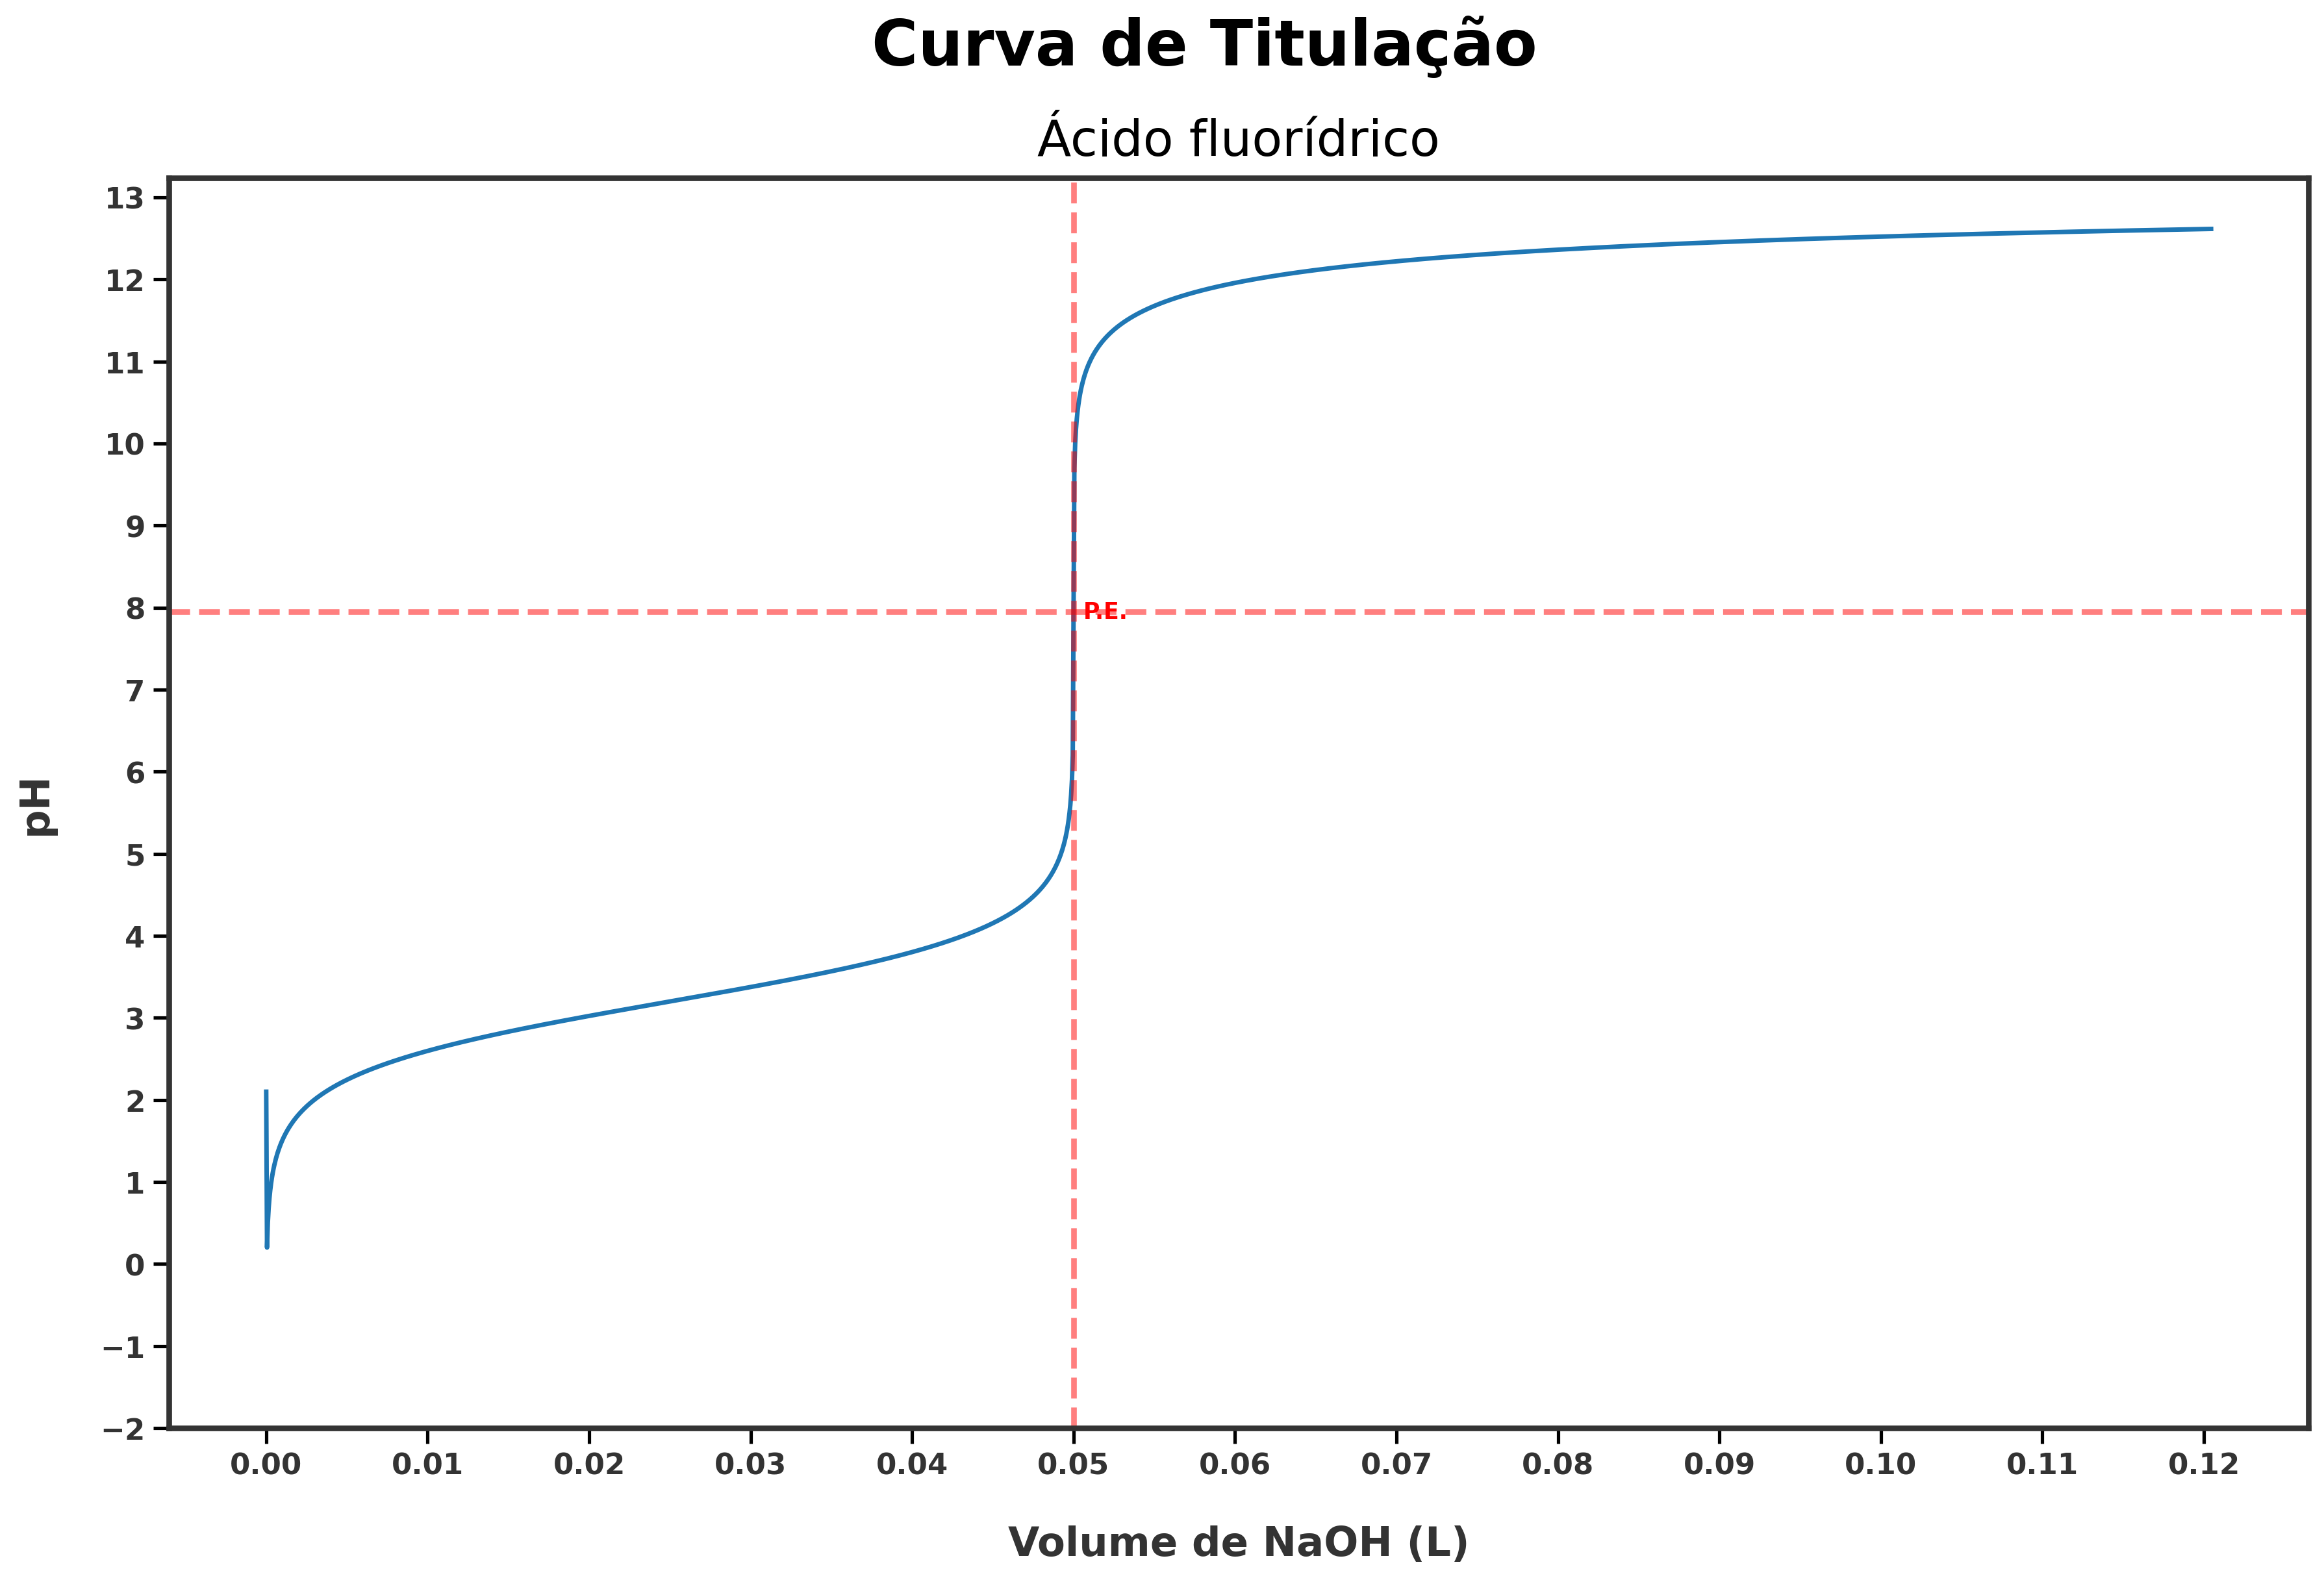
\includegraphics[width=0.9\linewidth]{curva/curva_de_titulacao_ácido_fluorídrico}
		\caption{}
		\label{fig:curvadetitulacaoácidofluorídrico}
	\end{subfigure}
	\begin{subfigure}{0.5\textwidth}
		\centering
		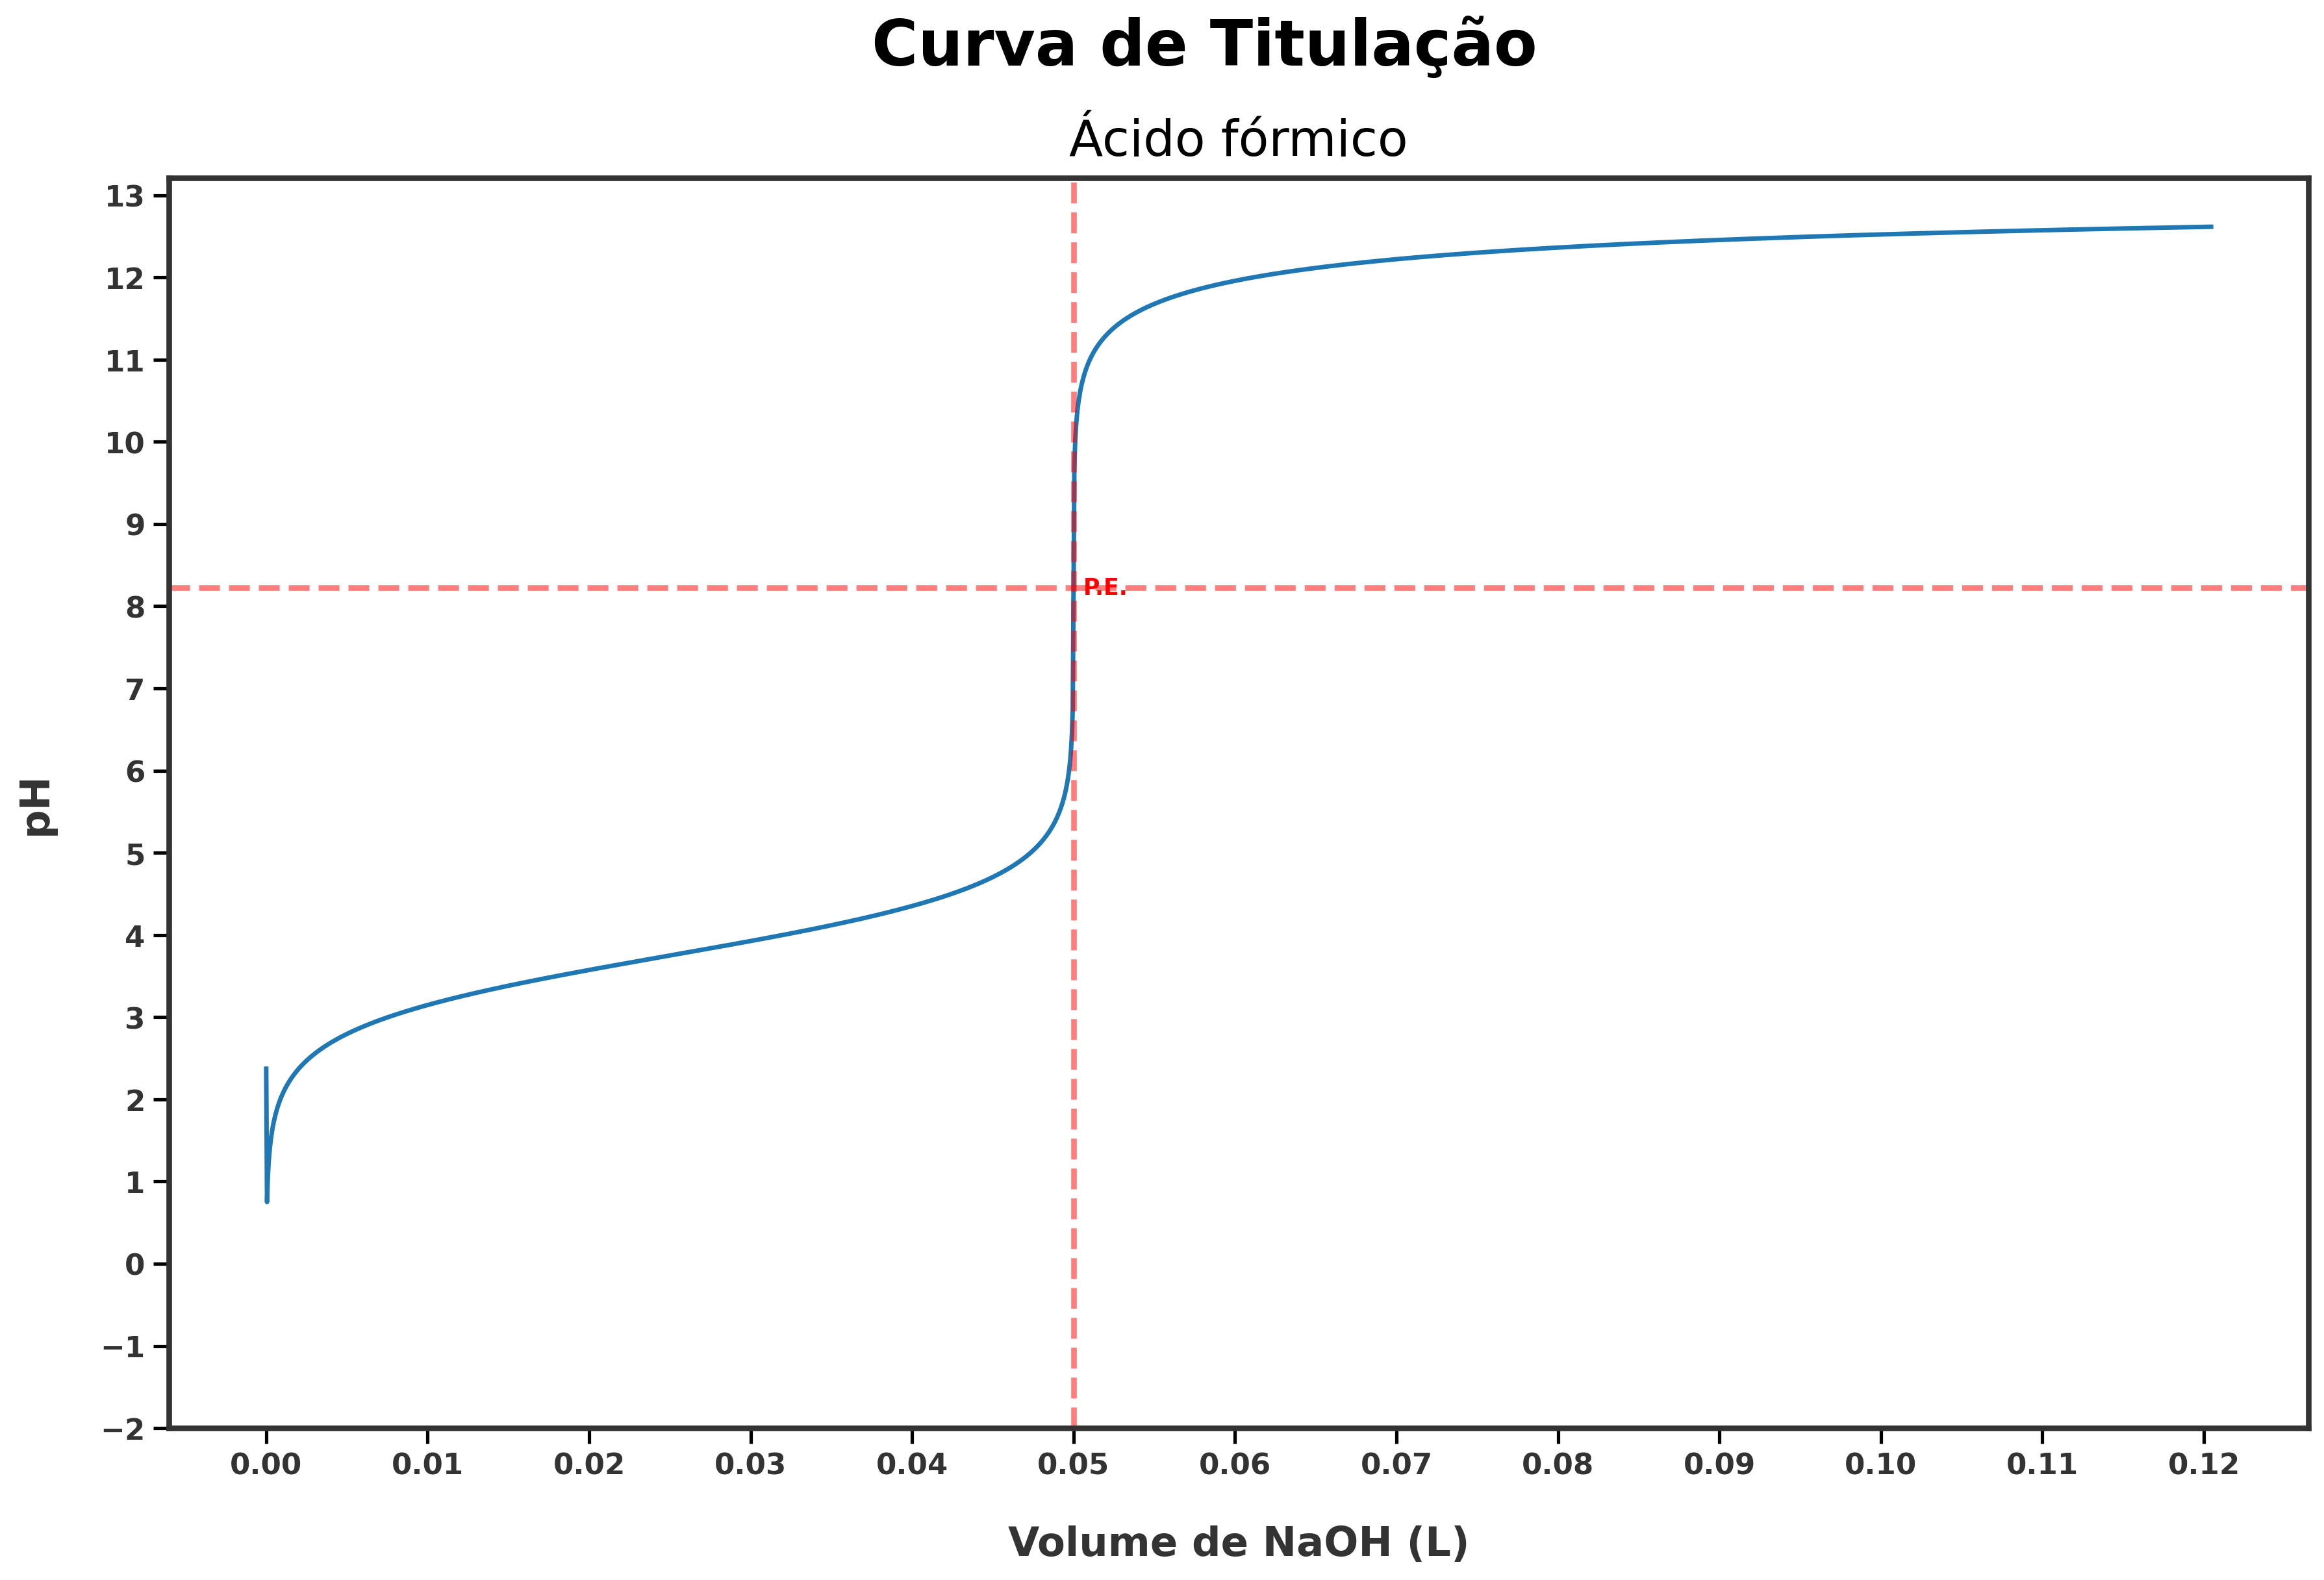
\includegraphics[width=0.9\linewidth]{curva/curva_de_titulacao_ácido_fórmico}
		\caption{}
		\label{fig:curvadetitulacaoácidofórmico}
	\end{subfigure}
	\begin{subfigure}{0.5\textwidth}
		\centering
		\includegraphics[width=0.9\linewidth]{curva/curva_de_titulacao_ácido_hidrazoico}
		\caption{}
		\label{fig:curvadetitulacaoácidohidrazoico}
	\end{subfigure}
\end{figure}
\begin{figure}
	\begin{subfigure}{0.5\textwidth}
		\centering
		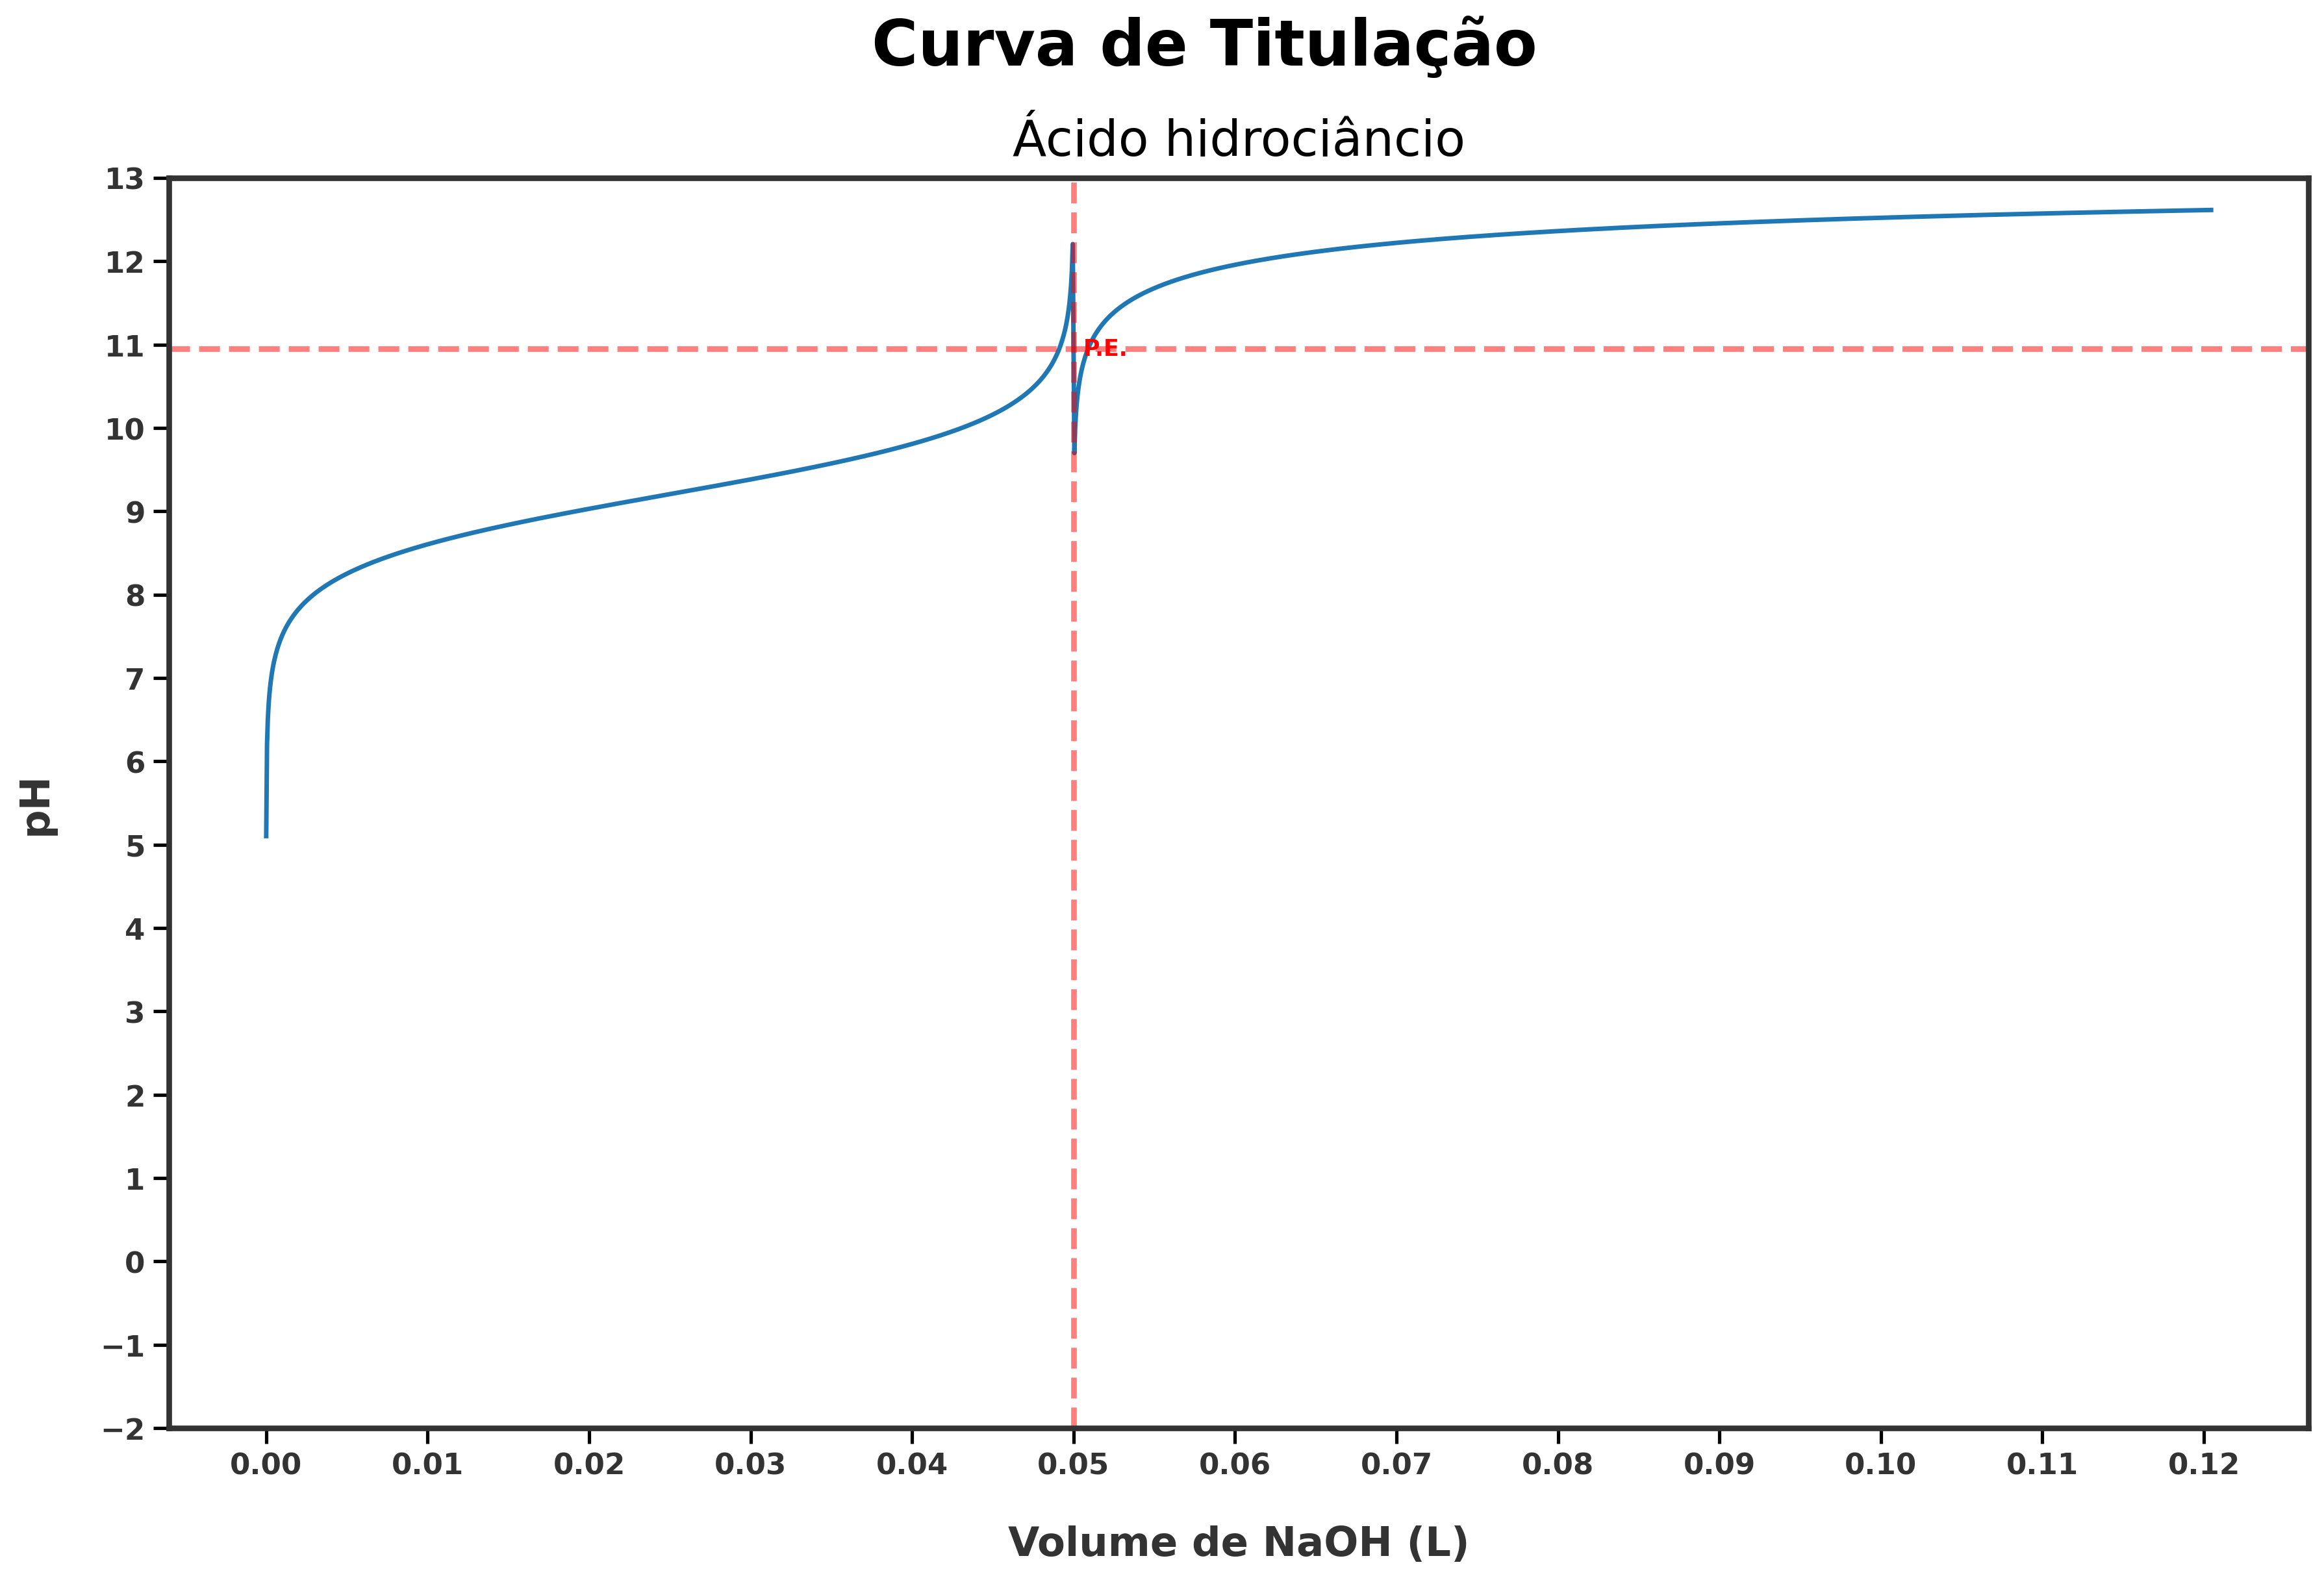
\includegraphics[width=0.9\linewidth]{curva/curva_de_titulacao_ácido_hidrociâncio}
		\caption{}
		\label{fig:curvadetitulacaoácidohidrociâncio}
	\end{subfigure}
	\begin{subfigure}{0.5\textwidth}
		\centering
		\includegraphics[width=0.9\linewidth]{curva/curva_de_titulacao_ácido_hipoiodoso}
		\caption{}
		\label{fig:curvadetitulacaoácidohipoiodoso}
	\end{subfigure}
	\begin{subfigure}{0.5\textwidth}
		\centering
		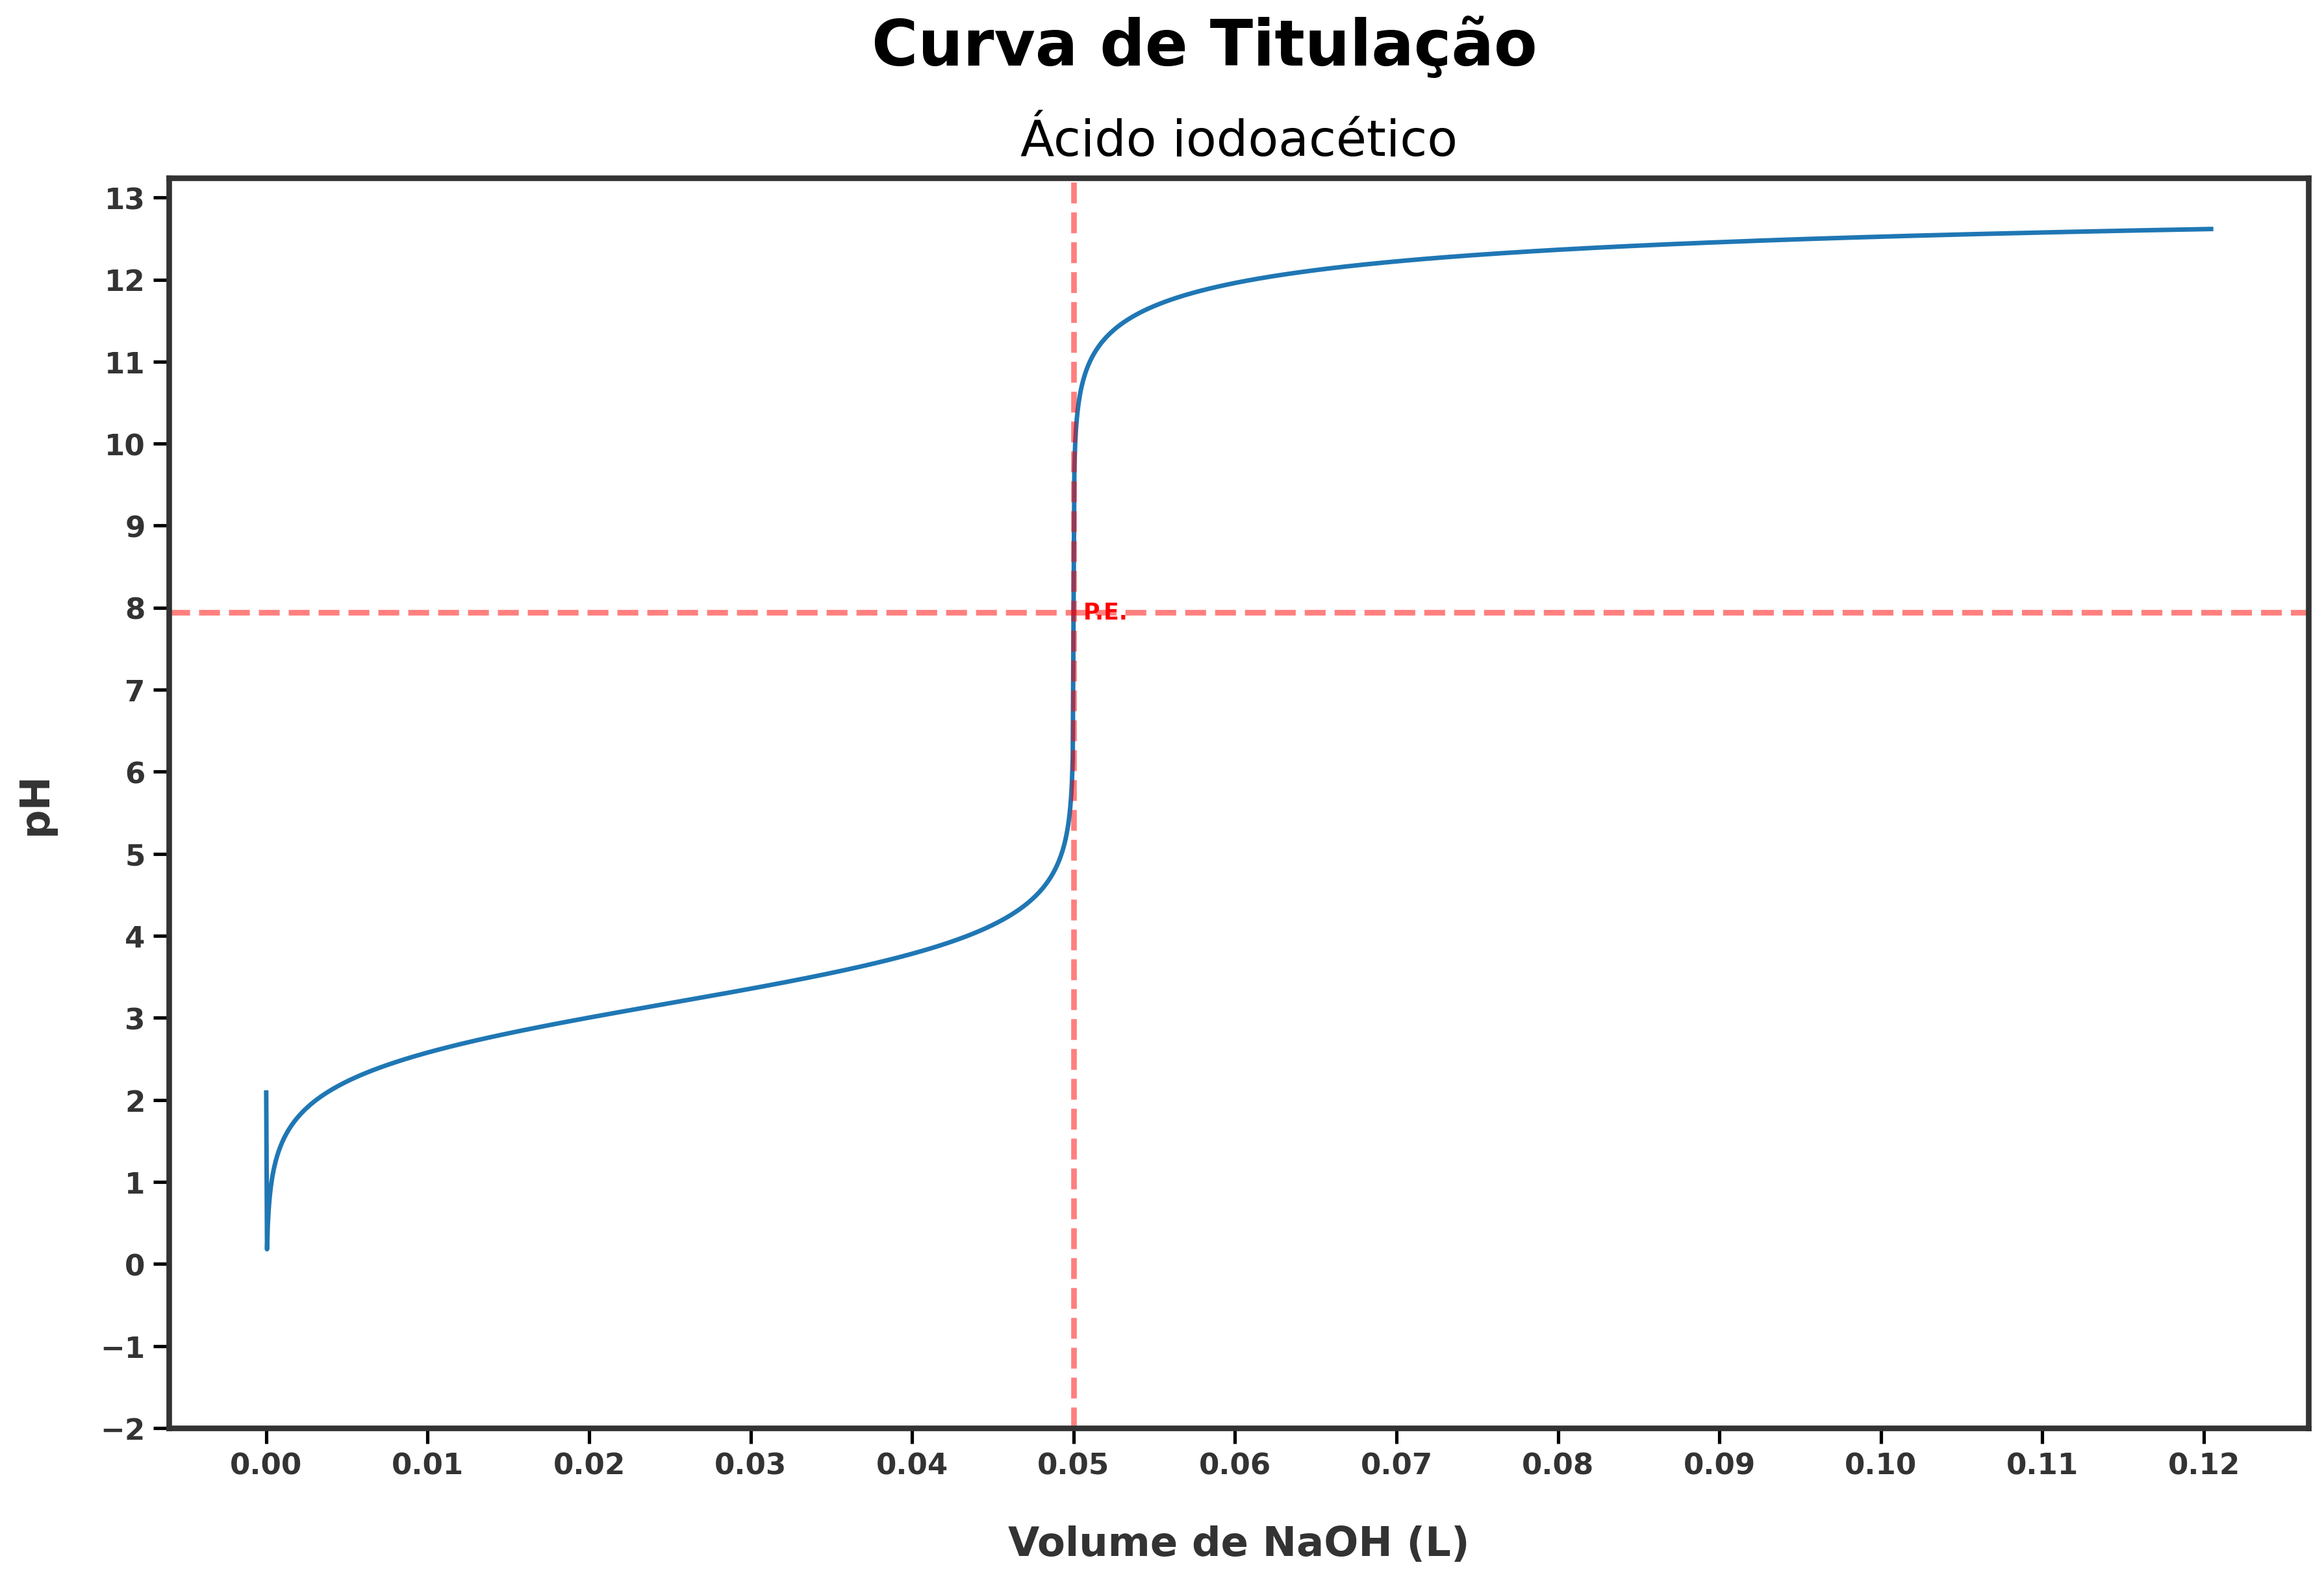
\includegraphics[width=0.9\linewidth]{curva/curva_de_titulacao_ácido_iodoacético}
		\caption{}
		\label{fig:curvadetitulacaoácidoiodoacético}
	\end{subfigure}
	\begin{subfigure}{0.5\textwidth}
		\centering
		\includegraphics[width=0.9\linewidth]{curva/curva_de_titulacao_ácido_nitroso}
		\caption{}
		\label{fig:curvadetitulacaoácidonitroso}
	\end{subfigure}
	\caption{Curvas de Titulação}
	\label{fig:curvas_de_titulacao}
\end{figure}
		

\end{document}